\documentclass{report}
\usepackage{graphicx}
\usepackage[utf8]{inputenc}
\usepackage{vmargin}
\usepackage[spanish]{babel}
%Options: Sonny, Lenny, Glenn, Conny, Bjornstrup
\usepackage[Sonny]{fncychap}
\usepackage[nottoc,numbib]{tocbibind}
\usepackage[section]{placeins}


\pagenumbering{arabic}



\begin{document}
    \begin{titlepage}
        \centering
        {
\includegraphics[width=1\textwidth]{images/logo_UCM}}
    
        \vspace{1cm}
        
        {\huge\textbf{TRABAJO DE FIN DE GRADO \\ }  }

        \vspace{0.5cm}
        
        {\huge\textbf{Esd2: Cuaderno de recogida de datos para el estudio médico}}
        
        \vspace{1.8cm}
    
        {\Large Eduardo Gonzalo Montero \\}
        \vspace{0.5cm}
        {\textbf \& \\}
        \vspace{0.5cm}
        {\Large Sergio Pacheco Fernández \\}
        
        \vspace{1.8cm}
        
        \raggedright
        {\Large \textbf{Profesor director:} Pablo Manuel Rabanal Basalo \\}
        \vspace{0.1cm}
        {\Large\textbf {Curso académico:} 2019-2020 \\}
        \vspace{0.1cm}
        {\Large\textbf {Identificación asignatura: }Grado de Ingeniería del Software \\}
   
        \clearpage
        
        \pagestyle{empty}
 
        \centering
        {
\includegraphics[width=1\textwidth]{images/logo_UCM}}
    
        \vspace{1cm}
        
        {\huge\textbf{FINAL DEGREE PROJECT \\ }  }

        \vspace{0.5cm}
        
        {\huge\textbf{Esd2: Cuaderno de recogida de datos para el estudio médico}  }
        
        \vspace{1.8cm}
    
        {\Large Eduardo Gonzalo Montero \\}
        \vspace{0.5cm}
        {\textbf \& \\}
        \vspace{0.5cm}
        {\Large Sergio Pacheco Fernández \\}
        
        \vspace{1.8cm}
        
        \raggedright
        {\Large \textbf{Director professor:} Pablo Manuel Rabanal Basalo \\}
        \vspace{0.1cm}
        {\Large\textbf {Academic year:} 2019-2020 \\}
        \vspace{0.1cm}
        {\Large\textbf {Subject identification: }Degree in Software Engineering \\}
    
        \clearpage
     \end{titlepage}

    \renewcommand{\contentsname}{Índice}
    \tableofcontents
    
    
    

\chapter*{Agradecimientos}
% Con esta línea el capitulo resumen aparecería en el índice
%\addcontentsline{toc}{chapter}{Agradecimientos}
    
    
    \textit{A todos los familiares, amigos y profesores que nos han acompañado en nuestro camino y nos han apoyado en momentos oscuros, que han compartido nuestra carga y han festejado nuestros éxitos, sin ellos no estaríamos aquí.
    A título personal, mención especial al profesor Antonio Navarro, sin el cual no habríamos llegado tan lejos y al que agradecemos todos los conocimientos adquiridos}.
    \newline
    
     \textit{“Si quieres ir rápido, ve solo. Si quieres llegar lejos, ve acompañado”}.
    \newline
    -Proverbio africano.
    \chapter*{Resumen}
\addcontentsline{toc}{chapter}{Resumen}

   Lorem ipsum dolor sit amet, consectetur adipiscing elit. Suspendisse venenatis consequat massa, vitae porttitor augue. Donec commodo ornare justo, vitae fermentum orci posuere sit amet. Curabitur vulputate sem odio, in tincidunt turpis venenatis vel. Nunc facilisis mi dui, tristique condimentum velit eleifend at. Nulla facilisi. Sed ac arcu sed ex convallis vestibulum eu et ante. Suspendisse sagittis eget nunc eget tempus. Nullam venenatis, felis non viverra volutpat, ex arcu lacinia magna, eget ullamcorper tellus sapien id magna.

Curabitur convallis tempus augue. Aliquam vehicula consectetur elit, ac porta arcu porttitor nec. Ut fringilla diam et est semper, at semper erat placerat. Sed in blandit magna, et suscipit lacus. Phasellus maximus libero vel libero ornare, vitae eleifend magna pellentesque. Vestibulum pharetra, arcu sit amet semper efficitur, lorem metus posuere nunc, in efficitur est nisi a neque. Pellentesque eu tellus urna.

In sit amet placerat sem. Donec sed efficitur velit. Sed at turpis eget tortor consequat consequat. Suspendisse et ullamcorper nibh. Phasellus dolor risus, tincidunt eget scelerisque eu, lacinia eget dui. Sed nibh lectus, tempor pharetra tempus sed, ultrices eget nisi. Fusce interdum, sapien ut accumsan blandit, urna sem suscipit lorem, in posuere enim lectus pharetra felis. Donec orci ligula, interdum facilisis lacinia in, venenatis et diam. Aliquam ut sem ut magna congue dapibus eget sed orci. Integer bibendum metus sit amet nisi dignissim elementum. Vestibulum imperdiet lacus enim. Ut at mauris et ipsum dapibus tincidunt. Nam id ipsum nec libero lobortis facilisis sit amet luctus ligula.
    \chapter*{Palabras clave}
\addcontentsline{toc}{chapter}{Palabras clave}

Lorem ipsum dolor sit amet, consectetur adipiscing elit. Suspendisse
     \chapter*{Abstract}
\addcontentsline{toc}{chapter}{Abstract}

   Lorem ipsum dolor sit amet, consectetur adipiscing elit. Suspendisse venenatis consequat massa, vitae porttitor augue. Donec commodo ornare justo, vitae fermentum orci posuere sit amet. Curabitur vulputate sem odio, in tincidunt turpis venenatis vel. Nunc facilisis mi dui, tristique condimentum velit eleifend at. Nulla facilisi. Sed ac arcu sed ex convallis vestibulum eu et ante. Suspendisse sagittis eget nunc eget tempus. Nullam venenatis, felis non viverra volutpat, ex arcu lacinia magna, eget ullamcorper tellus sapien id magna.

Curabitur convallis tempus augue. Aliquam vehicula consectetur elit, ac porta arcu porttitor nec. Ut fringilla diam et est semper, at semper erat placerat. Sed in blandit magna, et suscipit lacus. Phasellus maximus libero vel libero ornare, vitae eleifend magna pellentesque. Vestibulum pharetra, arcu sit amet semper efficitur, lorem metus posuere nunc, in efficitur est nisi a neque. Pellentesque eu tellus urna.

In sit amet placerat sem. Donec sed efficitur velit. Sed at turpis eget tortor consequat consequat. Suspendisse et ullamcorper nibh. Phasellus dolor risus, tincidunt eget scelerisque eu, lacinia eget dui. Sed nibh lectus, tempor pharetra tempus sed, ultrices eget nisi. Fusce interdum, sapien ut accumsan blandit, urna sem suscipit lorem, in posuere enim lectus pharetra felis. Donec orci ligula, interdum facilisis lacinia in, venenatis et diam. Aliquam ut sem ut magna congue dapibus eget sed orci. Integer bibendum metus sit amet nisi dignissim elementum. Vestibulum imperdiet lacus enim. Ut at mauris et ipsum dapibus tincidunt. Nam id ipsum nec libero lobortis facilisis sit amet luctus ligula.
    \chapter*{Keywords}
\addcontentsline{toc}{chapter}{Keyworlds}

\begin{itemize}
    \item Web service
    \item Medical research
    \item Diabetes
    \item Vitamin D
    \item API-REST
    \item Study
    \item Health
\end{itemize}

    
    \chapter{Introducción}
 En este capítulo se detalla la motivación que llevó a la realización del proyecto, los objetivos que este comprende y las pautas que se tomaron para lograr llevarlo a cabo
    
    \section{Objetivo}
    
    Este Trabajo de Final de Grado busca la implementación de un portal web que permita la recopilación de datos de interés para el estudio por parte del equipo médico. Para ello contará con formularios personalizados con los campos de interés  solicitados por el mismo que serán rellenados por los médicos en consultas rutinarias con los pacientes que hayan consentido participar en el proyecto. Estos datos serán luego accesibles tanto vía web como en archivos de Excel descargables desde el propio portal.\newline

	Con el fin de ajustar el producto final a las necesidades del equipo la aplicación se entregará con tiempo suficiente (aproximadamente en Febrero de 2020) para que pueda ser probada, revisada y modificada a medida. Esto es especialmente importante ya que el estudio se extenderá muchos meses más allá de la finalización de este TFG.\newline

	El objetivo final, y por supuesto el más importante, es que todo este desarrollo sirva de herramienta para ajustar los criterios de evaluación en los pacientes con diabetes mellitus tipo 2, permitiendo encontrar pautas en sus estados de salud subsanables que puedan en un futuro prevenir más casos de esta enfermedad.\newpage
	
	\section{Motivación}
    
    Nuestra primera motivación para adentrarnos en este proyecto son las tecnologías empleadas en el mismo. Ambos participantes están interesados en centrar su carrera en tecnologías web, uno de ellos trabajando ya de hecho como desarrollador full-stack. El proyecto da además libertad para ser implementado sin ningún tipo de restricciones de diseño o rendimiento, lo que plantea un escenario ideal para experimentar durante su desarrollo.\newline

	El otro motivo principal para decantarnos por este proyecto es su cercanía a un proyecto real. El cliente, la aplicación, los plazos y las necesidades del mismo no son algo creado para un ambiente académico, como otros desarrollos ya efectuados durante la carrera, sino un problema real que precisa una solución efectiva contando con todas las personas que lo acabarán utilizando. Además el proyecto requerirá de un mantenimiento post entrega, otro ámbito nunca explorado en la carrera y que será una valiosa experiencia de cara a nuestro futuro.\newline

	Por último remarcar que uno de los miembros, Sergio, ya tiene buenas experiencias con un proyecto anterior para el ámbito médico desarrollado en solitario para una empresa en Suiza y Eduardo siempre ha tenido interés en los hábitos de vida saludables y la nutrición, posible principal remedio para la diabetes extraído de los resultados de este estudio.\newpage
	
	\section{Metodología de trabajo}
    
    El proyecto será planificado bajo los estándares de la metodología Scrum\cite{Scrum} aunque distendiendo un poco sus cotas temporales, pues al ser solo dos miembros no es necesario hacer un hincapié tan diario en la organización para mantener el orden. Lo primero será definir cómo mantendremos los tres pilares básicos de la metodología: \textbf{transparencia, inspección y adaptación}.
    
    \begin{figure}[h]
    \centering
     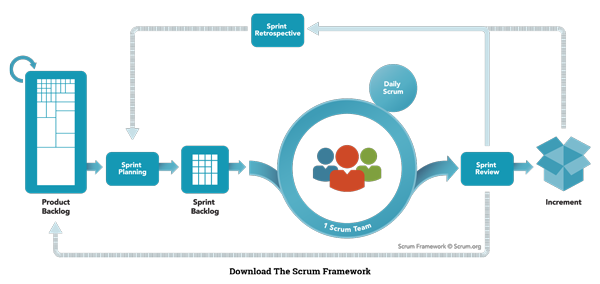
\includegraphics[width=1\textwidth]{images/Scrum.png}
    \caption{Flujo de trabajo en Scrum.}
    \end{figure}
    
    \subsection{Transparencia}
    Para mantener a ambos miembros al día de cualquier avance o variación en el proceso se empleará la herramienta online de Trello, que nos permitirá ir viendo en tiempo real los mismos. Este será estructurado de la siguiente forma:
    
    \begin{itemize}
    \item Se crearán dos columnas, una con la lista de tareas pendientes para el sprint actual y otra con las tareas actualmente en desarrollo. Además se creará una columna por cada sprint en la que se irán almacenando todas las tareas finalizadas. Cada tarea podrá encapsularse en una o más de estas categorías: despliegue, documentación, front, bug, investigación, modelo de datos, pendiente de resolver (cuestión a espera de la próxima reunión con el tutor), back, varios, resuelto (cuestiones ya solucionadas en anteriores reuniones que quedan como recordatorio). Además cada tarea llevará una o más etiquetas indicando los desarrolladores que han trabajado en ella.\newline
    
     \begin{figure}[h]
    \centering
     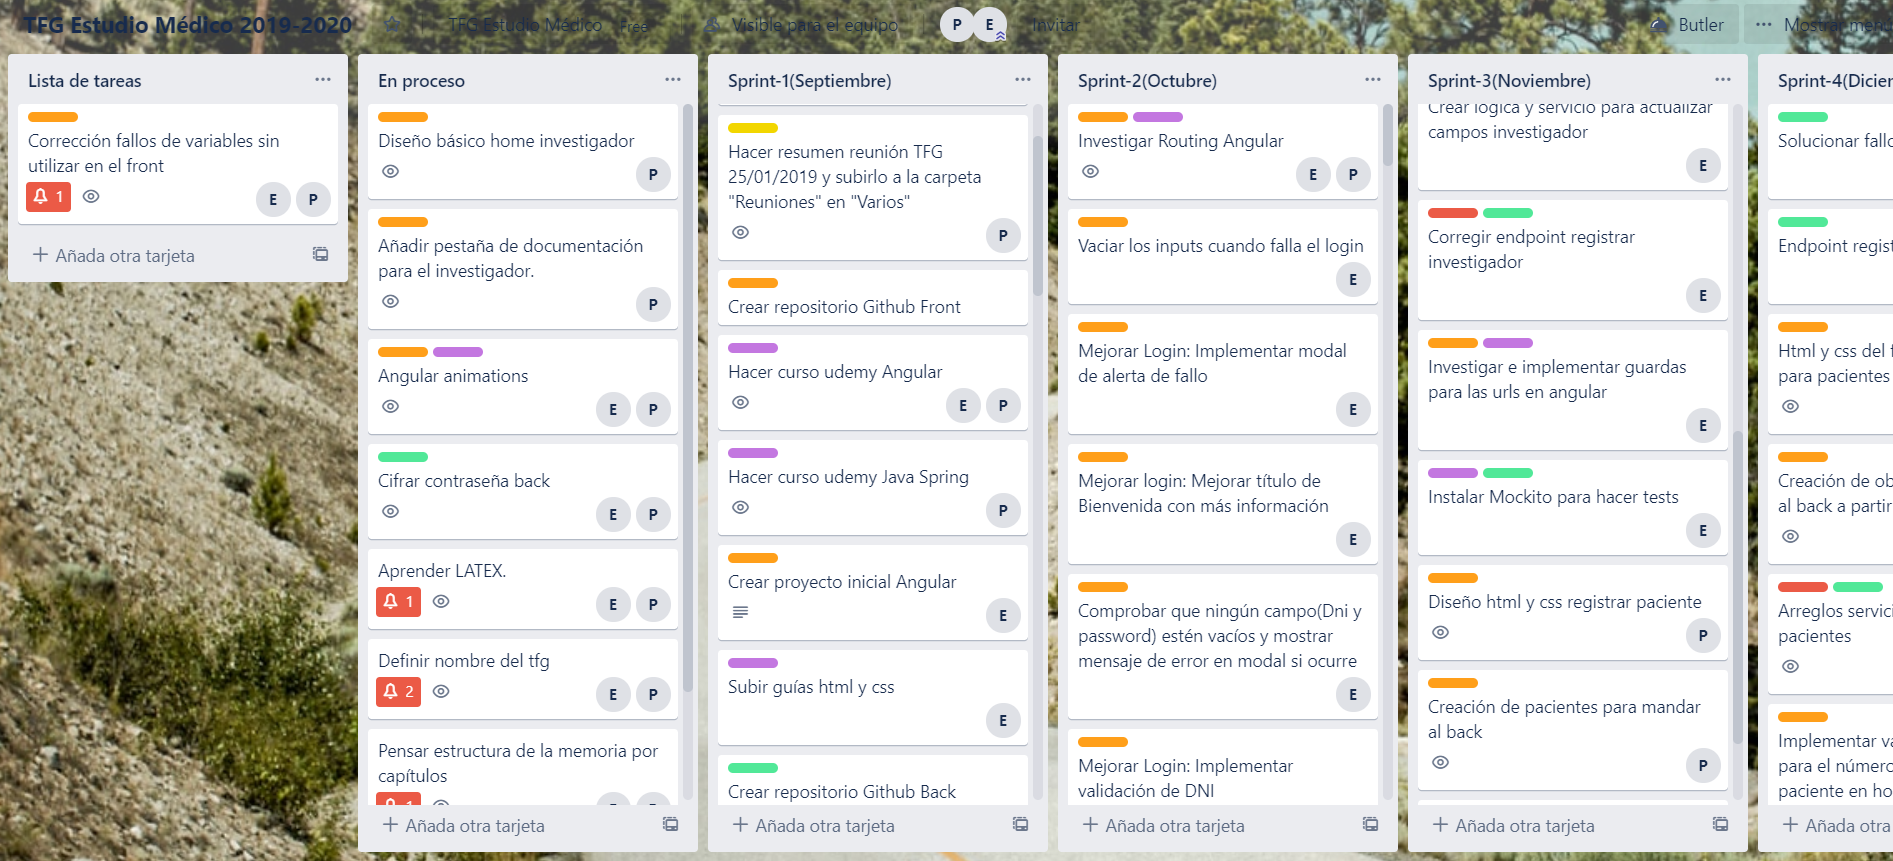
\includegraphics[width=1\textwidth]{images/Trello.jpg}
    \caption{Captura de ejemplo de la herramienta Trello.}
    \end{figure}
    \newpage
    
    \item  Asimismo, todo el código del proyecto estará subido y actualizado en un repositorio, en este caso GitHub\cite{github}, a traves del cual se podrá ver un histórico preciso de los cambios realizados en cada commit junto a comentarios explicativos del desarrollador que los haya realizado.\newline
    
    \begin{figure}[h]
    \centering
     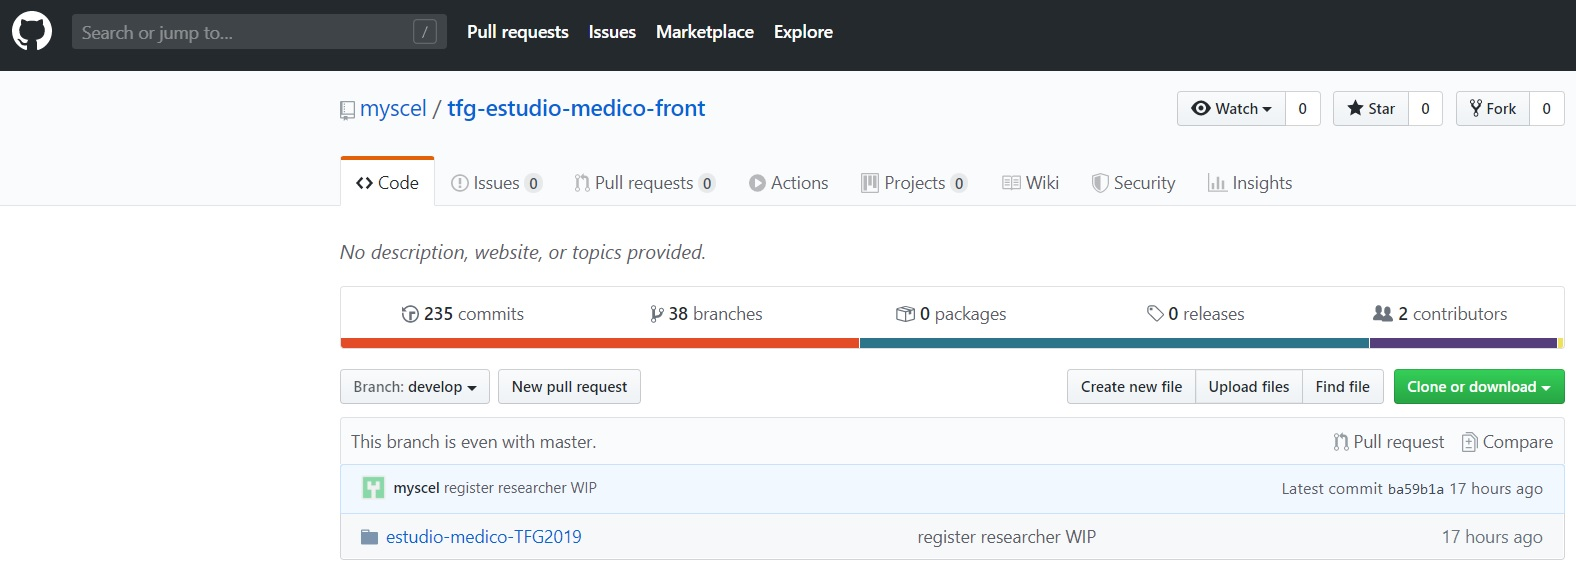
\includegraphics[width=1\textwidth]{images/GitHubFront.jpg}
    \caption{Captura de ejemplo del repositorio front en GitHub.}
    \end{figure}
    \end{itemize}
    
    \subsection{Inspección}
    Con el fin de mantener este principio, nuestro repositorio no solo albergará código, sino también un espacio separado para todos los artefactos derivados de Scrum, así como la documentación que se vaya creando durante el proceso que sea relevante a efectos de esta memoria. Estos artefactos serán por tanto accesibles constantemente por ambos miembros, los cuales avisarán en caso de cualquier añadido o modificación para que su compañero pueda revisarlo.\newline
    
    \begin{figure}[h]
    \centering
     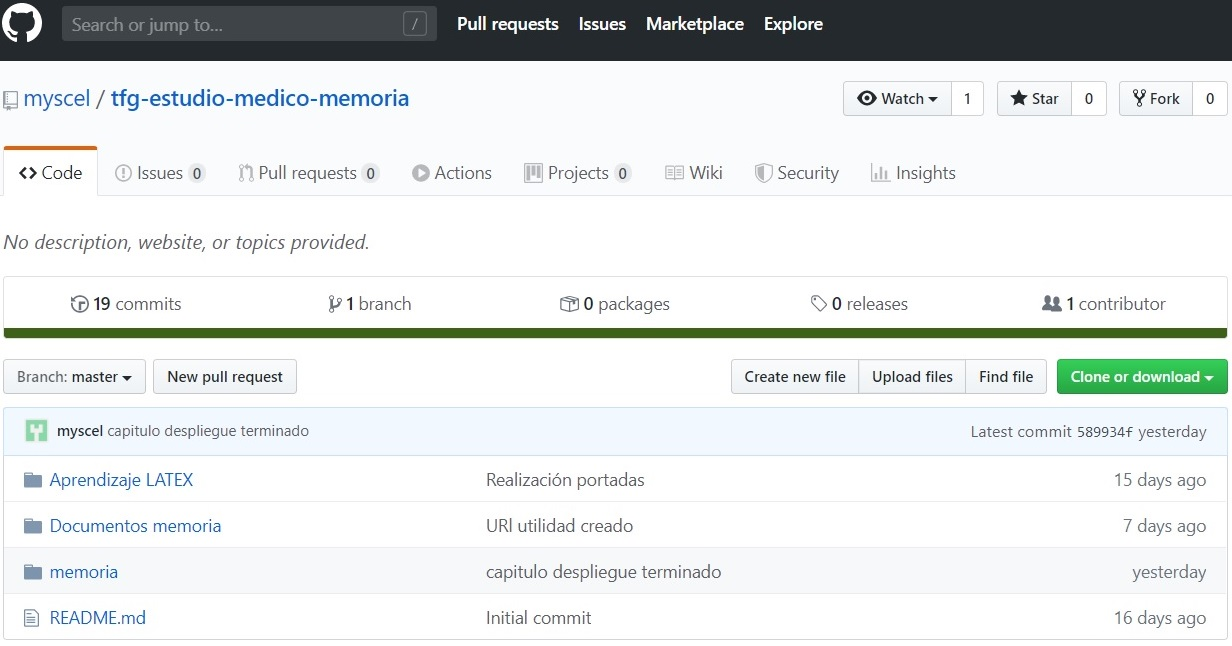
\includegraphics[width=1\textwidth]{images/GitHubMemoria.jpg}
    \caption{Captura de ejemplo con todos los documentos referentes a la memoria en GitHub tomada a posteriori.}
    \end{figure}
    \newpage
    
     \subsection{Adaptación}
    Al final de cada sprint se realizará una reunión tanto con el tutor del proyecto como con un representante del equipo médico para revisar el proceso y obtener feedback del mismo. Los errores o cambios urgentes extraídos de estas reuniones pasarán a ser la tareas más prioritarias del proyecto y su resolución será notificada de inmediato a ambos asistentes de la reunión. Además, para mantener el proyecto lo más afín a las necesidades del cliente cualquier cambio significativo en mitad de un sprint será notificado por correo previamente.
    \newline
    
    Además, de toda la documentación y artefactos mencionados disponibles durante el desarrollo los miembros mantendrán un contacto diario hablando de qué se ha hecho, se va a hacer y los problemas que se van encontrando, el cual hara las veces de Daily Scrums.\newline

	En cuanto a los roles típicos de Scrum, en nuestro caso, no serán utilizados. El Producto Owner será suplido con la comunicación directa y constante  de los miembros con el cliente que asegurará la priorización del valor para este durante el desarrollo. El Scrum Master no será preciso ya que ambos miembros del equipo tienen experiencia utilizando metodologías ágiles, tanto en la carrera como fuera en trabajos o proyectos propios. Por tanto solo existirá el equipo de desarrollo y este suplirá las funciones necesarias del resto de roles.\newline

	Los sprints serán de una duración mensual. Se opta por esta cuantía porque al estar uno de los miembros aún con clases y otro trabajando a jornada completa no se estima que en una semana el desarrollo pueda tener un avance suficientemente significativo. Estos sprints se iniciarán con una reunión de planificación con el tutor del proyecto y el representante del equipo médico, estipulando qué se hará y cómo. Asimismo, concluirán con otra reunión de misma índole que mostrará una demo funcional al representante y recogerá su feedback, para acto seguido comenzar con la reunión de planificación del siguiente sprint. Se decide aunar así el inicio y final del sprint en una sola reunión para evitar problemas de horarios difíciles de encajar por parte de los cuatro. Tras esta reunión con todos los miembros se realizará una pequeña reunión de retrospectiva solo del equipo de desarrollo para determinar si la metodología de trabajo funciona y qué se podría modificar o añadir.\newline

\chapter*{Introduction}
\addcontentsline{toc}{chapter}{1. Introduction}
This chapter details the motivation that led to the realization of this project, the objectives that it comprises and the guidelines that were taken to achieve it.


    \section*{1.1. Objective}
    \addcontentsline{toc}{section}{1.1. Objective}
    
    This Final Degree Project seeks the implementation of a web portal that allows the collection of data of interest for the study of the medical team. To do this, it will have personalized forms with the fields of interest requested by them, which will be filled in by doctors in routine appointments with patients who have consented to participate in the project. These data will then be accessible both via the web and in a downloadable Excel file from the portal itself.\newline
	
    In order to adjust the final product to the needs of the team, the application will be launched with 
    enough time (approximately in February 2020) so that it can be tested and modified to measure. This is especially important since the study will extend many months beyond the end of this TFG.\newline
	
	The final objective, and of course the most important one, is that all this development serves as a tool to adjust the evaluation criteria in patients with type 2 diabetes mellitus, allowing to find guidelines to improve in their life habits that may prevent more cases of this disease in the future.\newpage
	
	\section*{1.2. Motivation}
    \addcontentsline{toc}{section}{1.2. Motivation}
    
    Our first motivation to get into this project is the technologies used in it. Both participants are interested in focusing their career on web technologies, in fact one of them is already working as a full-stack developer. The project also gives freedom to be implemented without any design or performance restrictions, which presents an ideal scenario to experiment during its development.\newline
	
	The other main reason for opting for this project is its proximity to a real project. The client, the application, the deadlines and the needs of this project are not something created for an academic environment, like other developments already carried out during the degree, but a real problem that requires an effective solution with all the people who will end up using it. In addition, the project will require post-launch maintenance, another area never explored in the degree and which will be a valuable experience for our future.\newline
	
	Last but not least note that one of the members, Sergio, already has good experiences with a previous project in the medical field developed alone for a company in Switzerland and Eduardo has always had an interest in healthy lifestyle habits and nutrition, possible main remedy for diabetes extracted from the results of this study.\newpage

	\section*{1.3. Work methodology}
    \addcontentsline{toc}{section}{1.3. Work methodology}
    
    The project will be planned under the standards of the Scrum\cite{Scrum} methodology, although it will slightly loosen its temporary limits. Since there are only two members it is not necessary to place such daily emphasis on the organization to maintain order. The first thing will be to define how we will maintain the three basic pillars of the methodology: \textbf{transparency, inspection and adaptation}.
    
    \begin{figure}[h]
    \centering
     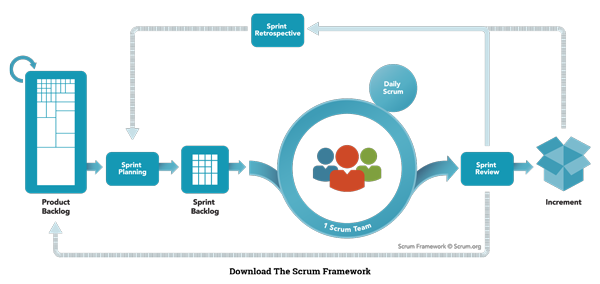
\includegraphics[width=1\textwidth]{images/Scrum.png}
    \caption{Workflow on Scrum.}
    \end{figure}
    
    \subsection*{1.3.1. Transparency}
    \addcontentsline{toc}{subsection}{1.3.1. Transparency}

    To keep both members up to date with any progress or variation in the process we will be using Trello's online tool, which will allow us to see them in real time. This will be structured in the following way:
    
    \begin{itemize}
    \item Two columns will be created, one with the list of pending tasks for the current sprint and another with the tasks currently in progress. In addition, a column will be created for each sprint in which all the completed tasks will be stored. Each task can be encapsulated in one or more of these categories: deployment, documentation, FrontEnd, bug, research, data model, pending resolution (questions for the the next meeting with the tutor), BackEnd, variety, resolved (questions already solved in previous meetings that stay as a reminder). In addition, each task will have one or more labels indicating the developers who have worked on it.\newline

    
     \begin{figure}[h]
    \centering
     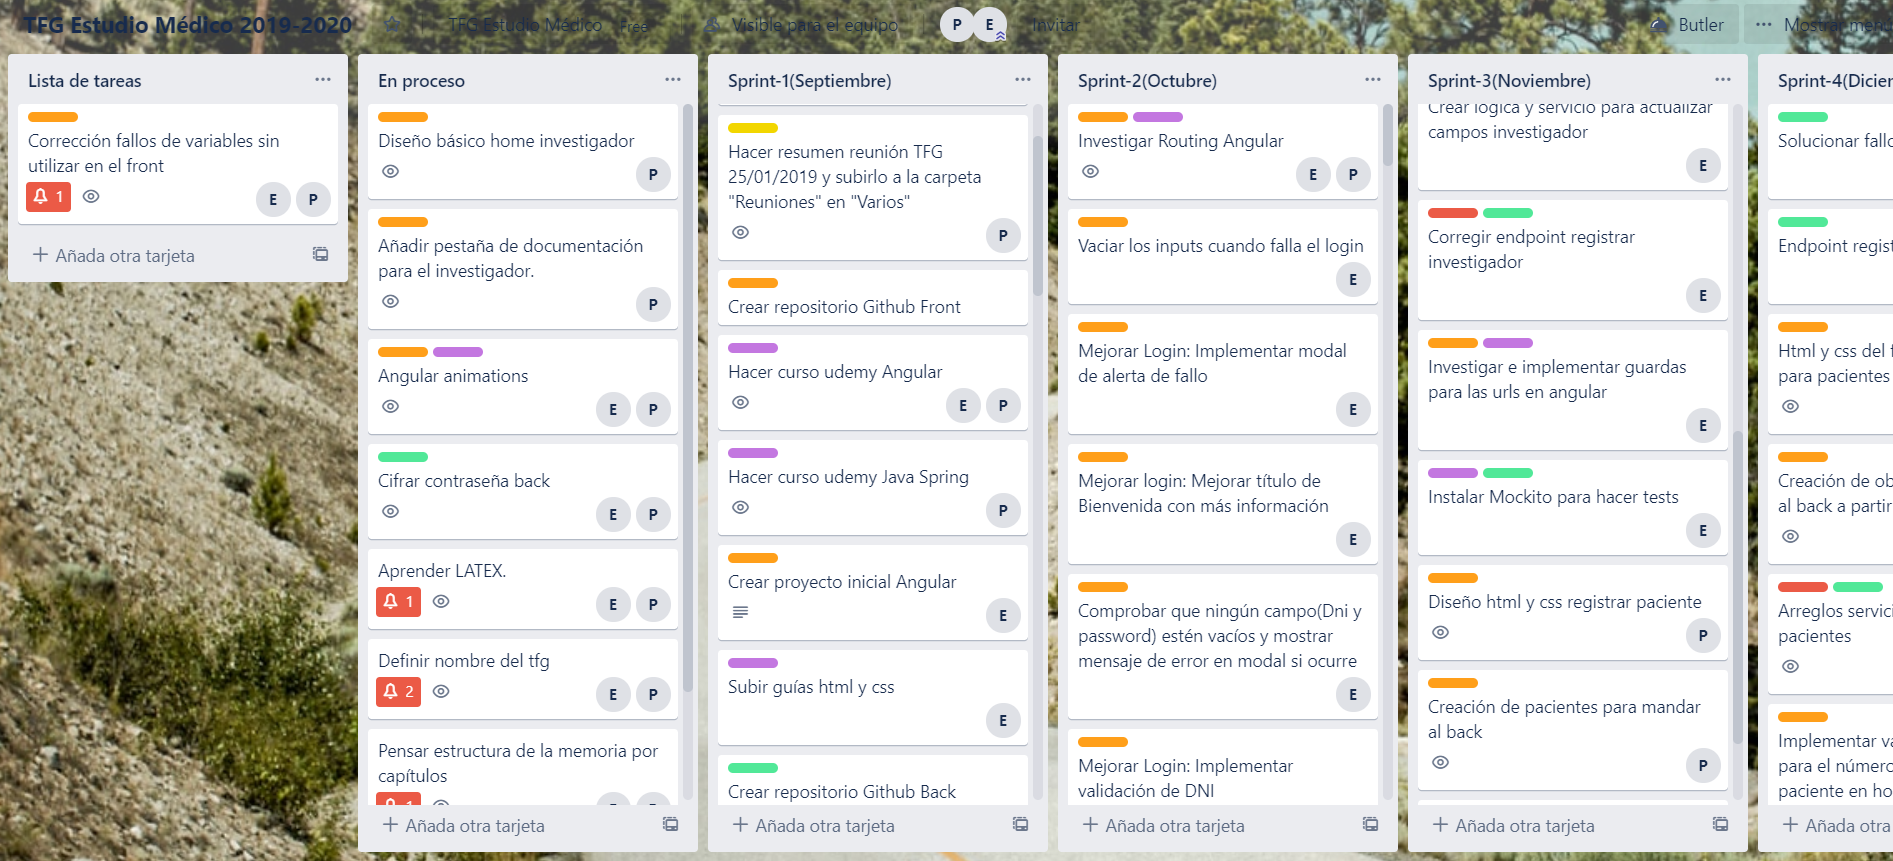
\includegraphics[width=1\textwidth]{images/Trello.jpg}
    \caption{Example image of Trello's online tool.}
    \end{figure}
    \newpage
    
    \item  Also, all the project code will be uploaded and updated in a repository, in this case GitHub\cite{github}, through which you can see an accurate history of the changes made in each commit along with explanatory comments from the developer that realised them.\newline

    \begin{figure}[h]
    \centering
     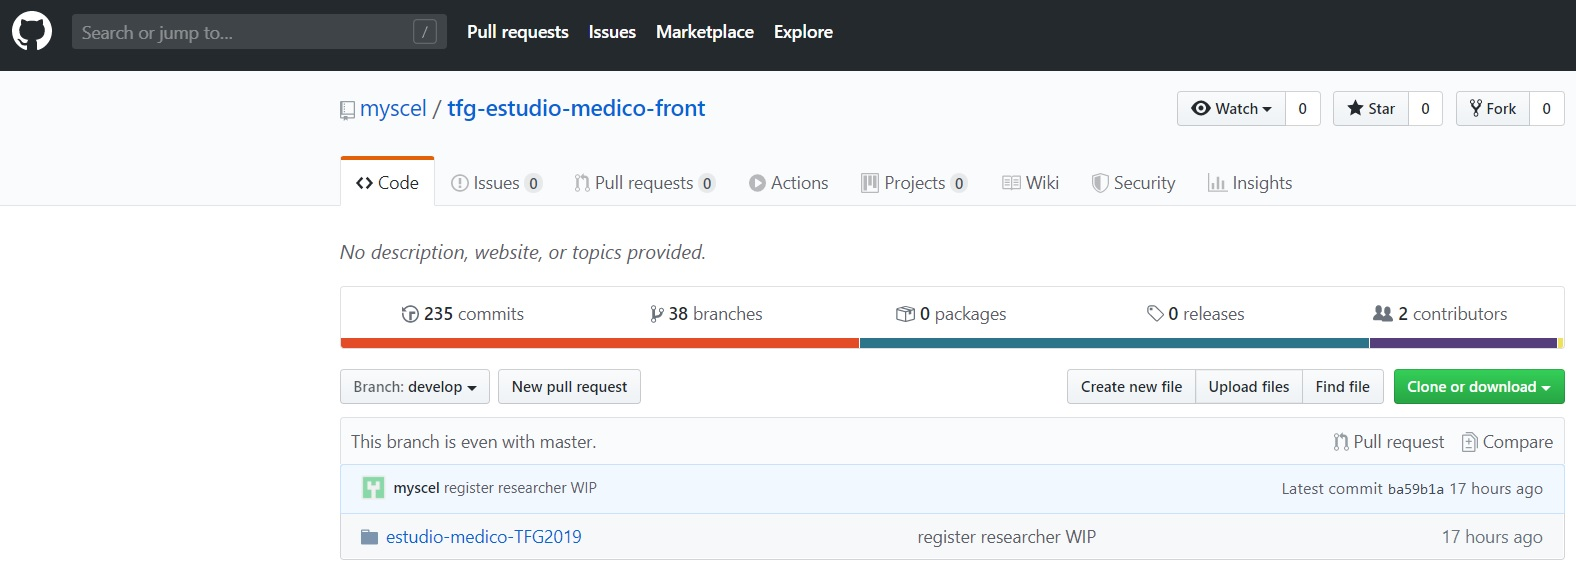
\includegraphics[width=1\textwidth]{images/GitHubFront.jpg}
    \caption{Example image of FrontEnd repository on GuitHub.}
    \end{figure}
    \end{itemize}
    
    \subsection*{1.3.2. Inspection}
    \addcontentsline{toc}{subsection}{1.3.2. Inspection}
    Con el fin de mantener este principio, nuestro repositorio no solo albergará código, sino también un espacio separado para todos los artefactos derivados de Scrum, así como la documentación que se vaya creando durante el proceso que sea relevante a efectos de esta memoria. Estos artefactos serán por tanto accesibles constantemente por ambos miembros, los cuales avisarán en caso de cualquier añadido o modificación para que su compañero pueda revisarlo.\newpage
    
    In order to uphold this principle, our repository will not only store code, but also a separate space for all the artifacts derived from Scrum, as well as the documentation that is created during the process that is relevant for the purposes of this report. These artifacts will therefore be constantly accessible by both members, who will notify in case of any addition or modification so that their partner can review them.\newline
    
    \begin{figure}[h]
    \centering
     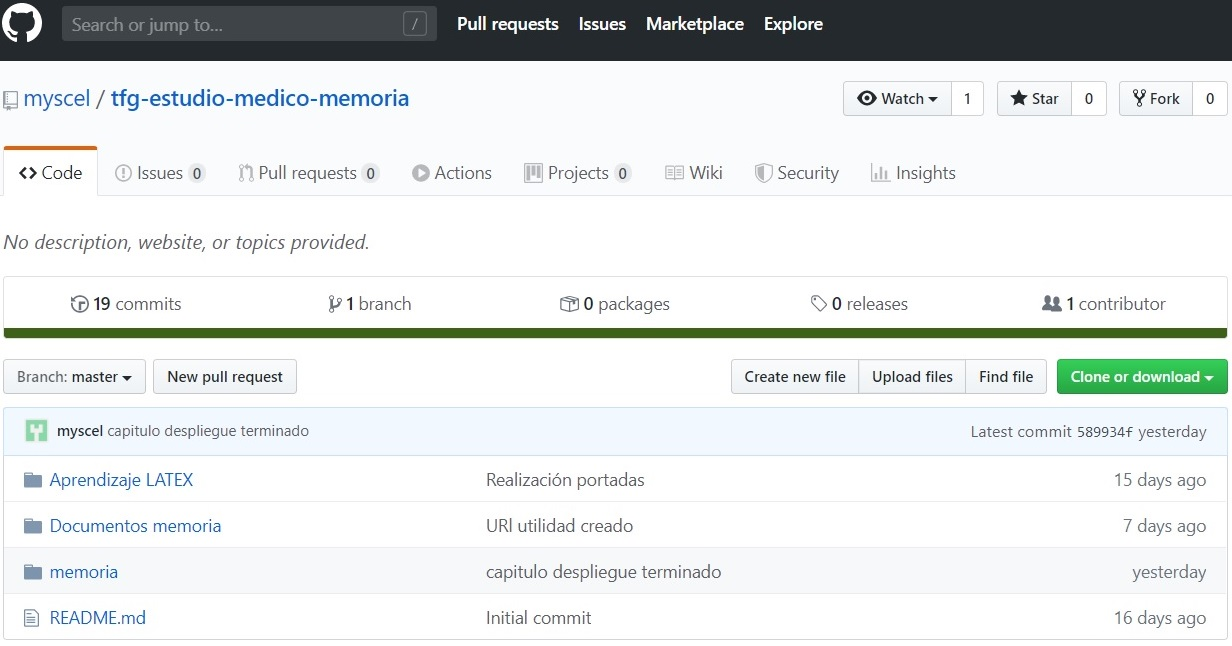
\includegraphics[width=1\textwidth]{images/GitHubMemoria.jpg}
    \caption{Example image of all the documents about this report on GitHub.}
    \end{figure}
    \newpage
    
     \subsection*{1.3.3. Adaptation}
    \addcontentsline{toc}{subsection}{1.3.3. Adaptation}
    
    At the end of each sprint there will be a meeting with both the project tutor and a representative of the medical team to review the process and obtain feedback on it. Errors or urgent changes extracted from these meetings will become the highest priority of the project and their resolution will be immediately notified to both meeting attendees. In addition, to keep the project as close as possible to the client's needs, any significant change in the middle of a sprint will be notified by mail in advance to them.\newline
    
    In addition of all the documentation and artifacts mentioned available during the development, the members will keep a daily contact talking about what has been done, what is going to be done and the problems they are encountering, which will act as Daily Scrums.\newline
	
	As for the typical Scrum roles, in our case, they will not be used. The Product Owner will be replaced with the direct and constant communication of the members with the client that will ensure the prioritization of the mos valuable features for the him during the development. The Scrum Master will not be precise since both team members have experience using agile methodologies, both in the career and outside in their own work or projects. Therefore, only the development team will exist and this will supply the functions for the rest of the roles.\newline
	
	Sprints will be monthly. This amount is chosen because one of the members is still with classes and the other is working full time, it is not estimated that in one week the development can have a  significant advance. These sprints will begin with a planning meeting with the project tutor and the medical team representative, stipulating what will be done. Likewise, they will conclude with another meeting of the same nature that will show a functional demo to the representative and collect their feedback, to then begin with the planning meeting for the next sprint. It was decided to combine the start and end of the sprint in a single meeting in order to avoid problems with schedules that were difficult for all four to fit into. After this meeting with all the members there will be a small retrospective meeting only for the development team to determine if the work methodology works and what could be modified or added.
    \chapter{Tecnologías}
 En este capítulo se detalla todo lo relativo a los lenguajes de programación, los entornos de desarrollo y los \textit{frameworks} elegidos para llevar a cabo este proyecto, así como sus características principales y la razón de su uso.
    
    \section{Lenguajes de programación}
    
    \subsection{TypeScript}
    TypeScript\cite{typescript} es un lenguaje de programación orientado a objetos (OO) el cual es un superconjunto de JavaScript. Decimos que una tecnología es un superconjunto de un lenguaje de programación, cuando puede ejecutar programas de la tecnología . En resumen, ejecutará el código como si fuese JavaScript. \newline
        
    TypeScript se diferencia de JavaScript principalmente en que posee inferencia de tipos, es decir, está fuertemente tipado, además de algunas funcionalidades extra.
    \newline
        
    Este lenguaje se utiliza en el \textit{frontend} del proyecto, dado que el \textit{framework} elegido para realizar esta parte es Angular, el cual se explicará en detalle más adelante.
        
    \subsection{HTML-5}
    HTML-5\cite{html} (HyperText Markup Language) es la quinta versión del lenguaje básico de la página web. Se trata de un lenguaje de marcación para la elaboración del contenido de las páginas web.
    Hoy en día es el lenguaje estándar que aceptan la gran mayoría de los navegadores a la hora de la construcción de las páginas web.
    \newline
     
    HTML-5 se diferencia de sus versiones anteriores en que incorpora nuevas etiquetas (section, article, header, footer etc...) con las cuales se busca mejorar y estandarizar la estructura de las páginas web además de otras actualizaciones como la mejora de los formularios o la inclusión de elementos de audio y vídeo.
    \newline
    
    Se ha optado por utilizar este lenguaje de marcación debido a su popularidad y a la inclusión de nuevas etiquetas que favorecen la lectura de la página web por parte de los navegadores.
    \newline
    
    \subsection{CSS-3}
    CSS\cite{css} (Cascading Style Sheets) es un lenguaje de diseño gráfico para gestionar el aspecto visual de un documento estructurado escrito en un lenguaje de marcación. Se utiliza en la mayoría de sitios web junto con HTML para generación de páginas web. De esta manera es mucho más sencillo generar páginas web, ya que, el diseño (CSS) se encuentra separado del contenido (HTML). \newline

    \subsection{Java 8}
    Java\cite{java} es un lenguaje de programación y una plataforma informática comercializada por primera vez en 1995 por Sun Microsystems\cite{sun} . Proviene de los lenguajes C y C++, y sus aplicaciones tienen la capacidad de ejecutarse en cualquier JVM (Java Virtual Machine).
    \newline
    
    Para este proyecto se ha utilizado la version 8 porque esta versión es la que menos \textit{bugs} tiene y la que mejora más la eficacia en el desarrollo y la ejecución de programas Java\cite{java8}. Además de estas razones, escogimos Java por ser un lenguaje orientado a objetos ideal para desarrollar proyectos \textit{API-REST}.
    
    \subsection{SQL}
    SQL\cite{sql} es un lenguaje declarativo estándar de comunicación dentro de las bases de datos que nos permite el acceso, gestión y manipulación de datos en una base de datos.
    \newline
    
    Se decidió utilizar este lenguaje debido a su uso en el SGDB (Sistema de Gestión de Base de Datos) que utilizamos en el proyecto, MySQL. Además de esto, SQL es ideal para trabajar con JPA (Java Persistence API) en el \textit{backend} del proyecto.
    
     \section{Entornos de desarrollo}
     
     \subsection{Visual Studio Code}
     Visual Studio Code\cite{vsc} es un editor de código fuente desarrollado por Microsoft para Windows, Linux y macOS. Incluye, entre otras características, soporte para el proceso de depurar, finalización inteligente de código o refactorización de código.
    \newline
    
    En este proyecto se ha utilizado este entorno de desarrollo para gestionar un proyecto Angular, ya que este editor posee gran versatilidad a la hora de instalar plugins y gestionar diferentes lenguajes de programación de manera simultánea.
    
     \subsection{MySQL Workbench}
     MySQL Workbench\cite{mysql} se trata de un programa para gestionar, diseñar y administrar bases de datos relacionales, utilizado en nuestro proyecto a la hora de manejar datos de manera local. \\
     \newline
     Se decidió utilizar debido a que se ha usado previamente en nuestros estudios de grado en diversas asignaturas de manera productiva, además de que posee una versión gratuita.
     
     \subsection{PhpMyAdmin}
     Al igual que MySQL Worbench, se trata de una herramienta de gestión de bases de datos MySQL, pero con la diferencia que el acceso a esta herramienta es vía web, alojándose en un servidor.\\
     \newline
     Esta herramienta la utiliza Hostinger\cite{hostinger},  proveedor de alojamiento web donde se ha decidido alojar el proyecto para desplegarlo en la web.
     
     \subsection{GitHub}
     GitHub\cite{github} es un sistema de gestión de proyectos y control de versiones de código que funciona con git, el cual hemos utilizado para trabajar en equipo. \\
     \newline
     Se decidió utilizar este sistema debido a la familiaridad que poseemos con el mismo, lo que se traduce en efectividad y productividad en el flujo de trabajo del equipo.
     
 

     \subsection{Bitbucket}
     Bitbucket\cite{bitbucket} es, al igual que GitHub, un sistema de gestión de proyectos y control de versiones. No se tenía planificado utilizar este sistema, pero un cambio en la política de GitHub por el cual se nos impedía gestionar nuestros repositorios de manera privada entre otros cambios, nos obligó a buscar otras opciones con versiones gratuitas en las cuales guardar una copia auxiliar del proyecto en caso de que algo fallase con GitHub.
     \newline
     
     Tras una búsqueda de sistemas similares, nos decantamos por utilizar Bitbucket debido a la posibilidad de crear repositorios privados gratuitos e ilimitados para equipos pequeños (menos de 5 personas). \newline
     
     \subsection{Eclipse}
     Eclipse\cite{eclipse} es una plataforma de software formado por herramientas \textit{open source} para el desarrollo de aplicaciones.
     \newline
     
     A lo largo de nuestro paso por los estudios de grado en Ingeniería del Software, hemos utilizado este programa para desarrollar código, razón por la cual lo hemos escogido para la realización de la parte \textit{backend} del proyecto.
     
     
     \subsection{Overleaf}
     Overleaf\cite{overleaf} es un gestor online de proyectos escritos en \LaTeX. Gracias a los cursos formativos impartidos por la Oficina de Software Libre\cite{ucmsoftwarelibre} realizado en años anteriores y a los recursos puestos a disposición de los alumnos\cite{recursoslatex} nos animamos a realizar la memoria con este editor online y en lenguaje de maquetación \LaTeX.
     
     
         \subsection{MobaXterm}
     MobaXterm\cite{mobaxterm} es una herramienta muy versátil, entre sus funciones destacan la emulación de terminales o la conexión a un cliente SSH.
     \newline 
     
     En este proyecto lo utilizamos con el objetivo de conectarse al servidor remoto proporcionado por Hostinger\cite{hostinger}, en el cual albergamos el despliegue de la parte \textit{backend} de nuestro proyecto.\newpage
     
     
     \section{Frameworks}
     
     \subsection{Java Spring}
     Spring\cite{javaspring} es un \textit{framework} del lenguaje de programacion Java el cual nos permite desarrollar aplicaciones de manera más rápida, eficaz y corta, saltándonos tareas repetitivas y ahorrándonos líneas de código.
     \newline
     
     Una de las características que define  Java Spring de otros \textit{frameworks} es la inversión de control, por la cual, es el \textit{framework} y no el programador el que ejecuta ciertas operaciones sobre la aplicación, invirtiendo de esta manera los métodos de programación tradicionales.
     Otra de las características propias de Java Spring es la inyección de dependencias, por la cual Spring es capaz de crear o instanciar aquellos objetos que el programador necesite, favoreciendo el desacoplamiento y la manejabilidad de los mismos.
     Además de esto da soporte a una gran cantidad de \textit{frameworks} a través de dependencias, facilitando la tarea del programador.
     \newline
     
     Hemos escogido este \textit{framework} para realizar la parte \textit{backend} de nuestra aplicación por las características citadas anteriormente, construyendo una \textit{API-REST}. Esta \textit{API-REST} actúa como un servidor, siendo consumida por un cliente.
     \newline
    
    Spring da soporte a una gran cantidad de herramientas a través de dependencias. Dichas dependencias se gestionan mediante Maven\cite{maven}, una herramienta que simplifica los procesos de instalación.
    
    \begin{figure}[h]
    \centering
    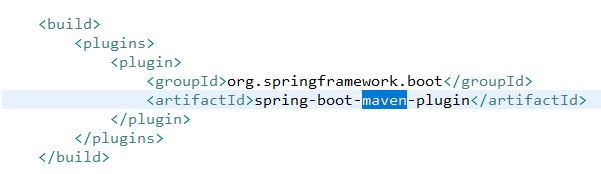
\includegraphics[width=1\textwidth]{images/maven}
    \caption{Instalación Maven en Java Spring}
    \end{figure}
    
    

        \subsubsection{\underline{Swagger}}
        Swagger\cite{swagger} es un proyecto \textit{open source} para describir, gestionar, consumir y visualizar aplicaciones \textit{API REST.} Para este proyecto vamos a utilizarlo con código Java, con el objetivo de generar la documentación de los puntos de acceso y de las entidades que se envían y se reciben.

        
        \subsubsection{\underline{Mockito}}
        Mockito\cite{mockito} es un \textit{framework} utilizado junto con JUnit\cite{junit} en Java para realizar tests de manera sencilla. En este proyecto se va a utilizar para testear las capas de \emph{Business} y \emph{Controller}, con el objetivo final de conseguir un 100\% de cobertura en las clases testeadas.
        \newline
        

        \subsubsection{\underline{JPA}}
        JPA\cite{jpa} (Java Persistence API) es una especificación de Java para acceder, persistir y gestionar datos entre Clases-Objetos de Java y bases de datos relacionales.
        \newline
        
        Gracias a los conocimientos de JPA adquiridos y desarrollados en las asignaturas de IS (Ingeniería del Software) y MS (Modelado de Software), nos decantamos por esta opción para gestionar las llamadas a las bases de datos correspondientes.
        

     \subsection{Angular}
       Angular\cite{angular} es un \textit{framework} de desarrollo de aplicaciones SPA (Single Page Applications), el cual utiliza Typescript como lenguaje de programación. Este \textit{framework} tiene la ventaja de que no refresca el navegador al modificar los elementos de la página web, dando una sensación de dinamismo y de inmersión al usuario.
       \newline
       
       Nos decantamos por utilizar este \textit{framework} debido a su popularidad y al gran uso que se le da a nivel empresarial.

        \subsubsection{\underline{Bootstrap}}
         Bootstrap\cite{bootstrap} es una herramienta para crear interfaces de usuario limpias y totalmente adaptables a todo tipo de dispositivos y pantallas, sea cual sea su tamaño.
         \newline
         
         Escogimos esta herramienta ya que nos proporciona resultados óptimos y limpios de manera rápida, además de que posee una extensa documentación\cite{documentationboostrap} a la que acudir en caso de duda.

   
     
    \chapter{Despliegue}
    En este capítulo se detalla como, una vez terminada una versión final de la aplicación, se comienza con el proceso de habilitar el uso de la aplicación desde la web. Para ello decidimos utilizar la pataforma Hostinger\cite{hostinger}, y todos los servicios que la misma proporciona a sus usuarios.
    \newline
    
    El despliegue de la aplicación consta de tres partes; el despliegue de la aplicación FrontEnd, el despliegue de la aplicación BackEnd, y el despliegue de la base de datos.
    
    \section{FrontEnd}
    Para desplegar la aplicación Angular que representa el FrontEnd de nuestra aplicación, se utilizó la herramienta ``Administrador de archivos'' que nos ofrece Hostinger y que nos proporciona una interfaz de usuario para administrar archivos y directorios en nuestro dominio \textit{tfg-estudio-medico.com}.
    \newline
    
    En dicho administrador, se procedió a subir la carpeta \textit{dist} generada por el proyecto Angular.
    
     \begin{figure}[h]
    \centering
     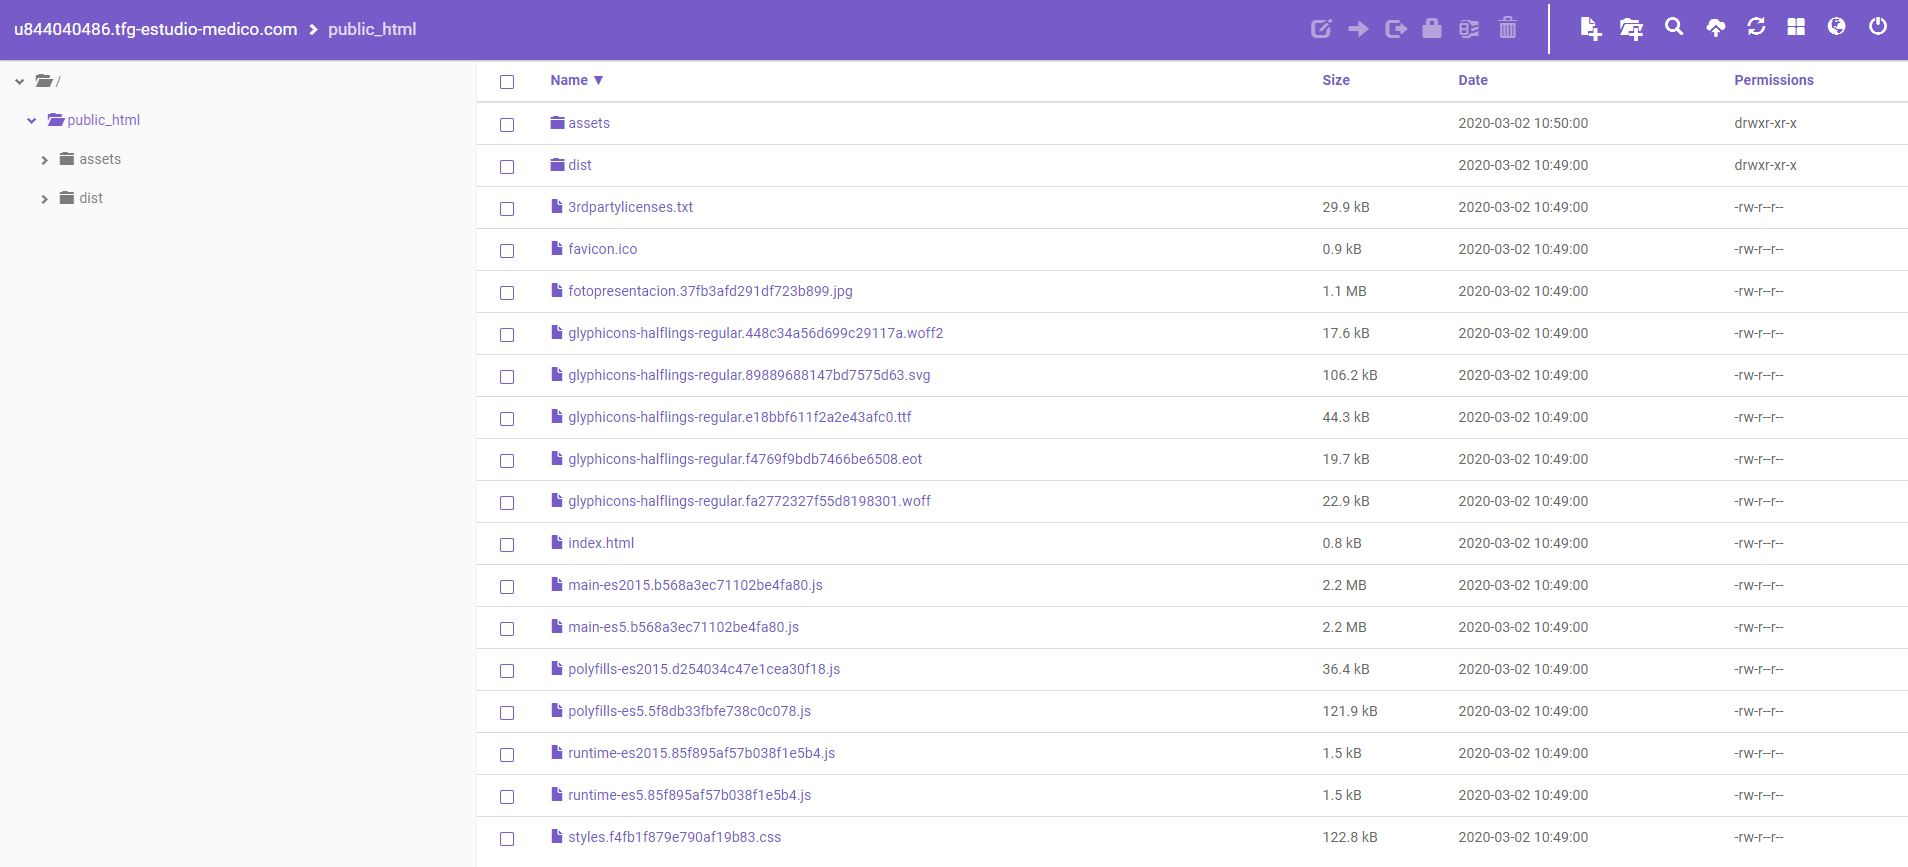
\includegraphics[width=1\textwidth]{images/administradorarchivos}
    \caption{Administrador de archivos de Hostinger}
    \end{figure}
    

    \section{BackEnd}
    Para desplegar la aplicación Java Spring que constituye el BackEnd de nuestra aplicación, se utilizó un servidor proporcionado por Hostinger\cite{hostinger}. En dicho servidor instalamos un sistema operativo Ubuntu 18.04 64bit.
    
     \begin{figure}[h]
    \centering
     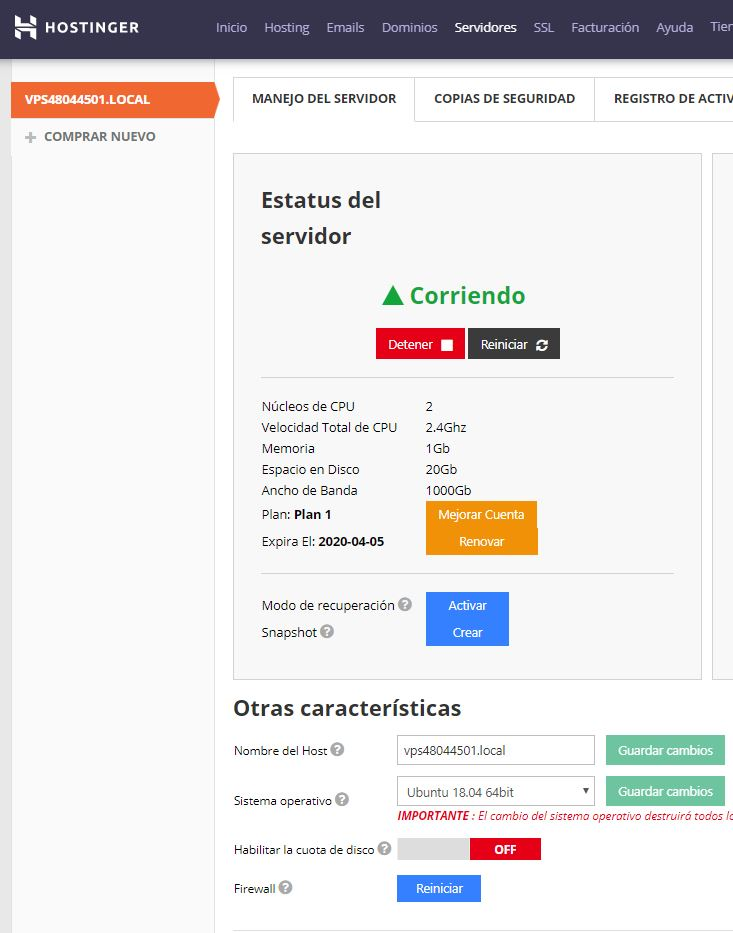
\includegraphics[width=0.4\textwidth]{images/servidorhostinger}
    \caption{Servidor en Hostinger}
    \end{figure}
    
    \FloatBarrier
    
    Para conectarnos al servidor utilizamos el programa MobaXterm, conectándonos al servidor a traves de SSH. Nuestro objetivo era mantener el archivo .jar ejecutándose en la máquina incluso si no estamos conectados a la misma, para ello generamos un \textit{servicio}, esto es, un script que se mantiene arrancado incluso si cerramos la sesión. \\
    \newline
    Lo primero que tenemos que hacer es generar el archivo ejecutable de nuestro proyecto BackEnd. Una vez generado el archivo SNAPSHOT .jar de nuestro proyecto Java Spring, nos disponemos a subirlo a la carpeta /root/back.
    
    \begin{figure}[h]
    \centering
     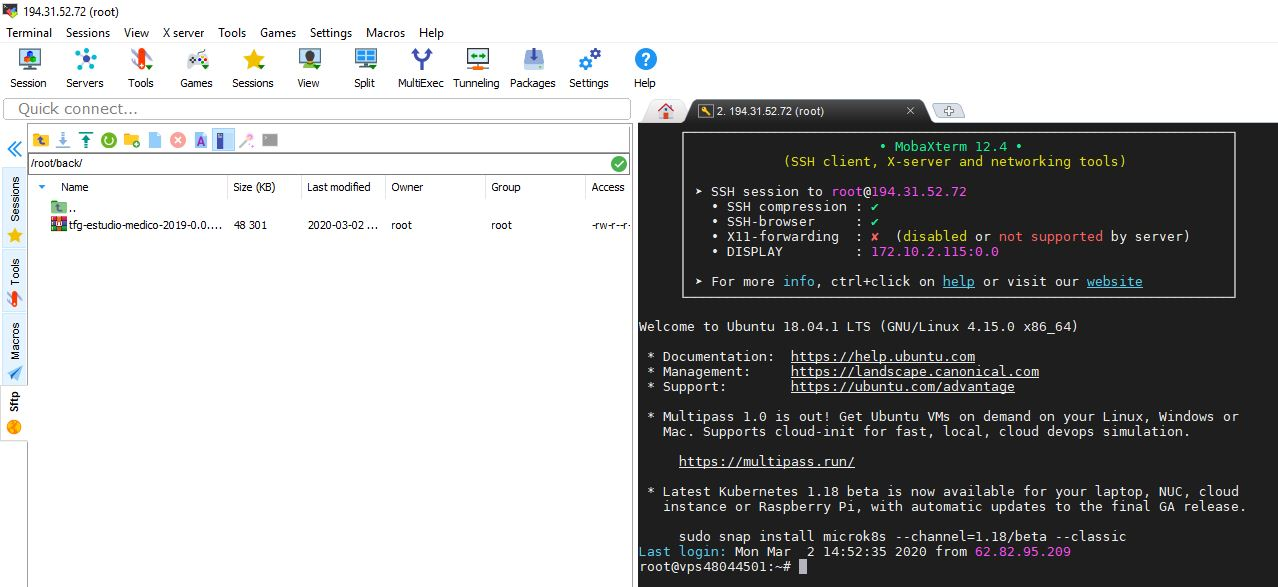
\includegraphics[width=0.9\textwidth]{images/jarback}
    \caption{Jar desplegado en MobaXterm}
    \end{figure}
    
    A continuación, generamos un script llamado \textit{start\_back.sh}  que simplemente ejecuta el comando \textit{java -jar} para arrancar el ejecutable .jar, el cual vamos a guardar en el directorio /usr/local/bin. Lo guardamos en dicho directorio debido a que este directorio es accesible por todos los usuarios.
    
    \begin{figure}[h]
    \centering
     
\includegraphics[width=1\textwidth]{images/script}
    \caption{Script start\_back.sh desplegado en MobaXterm}
    \end{figure}
    
    Después hemos generado un \textit{servicio} llamado \textit{daemonback.service} en la carpeta /etc/systemd/system, que es el directorio indicado en sistemas Linux para almacenar y gestionar demonios. Este servicio se encarga de ejecutar en segundo plano el script \textit{start\_back.sh}. 
    
    \begin{figure}[h]
    \centering
     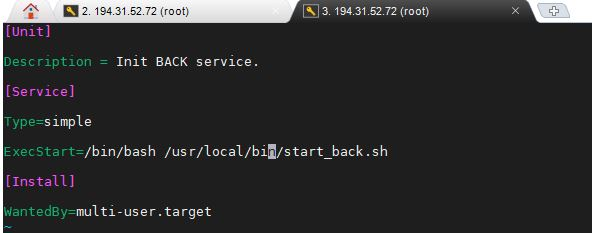
\includegraphics[width=1\textwidth]{images/demonio}
    \caption{Servicio daemonback.service desplegado en MobaXterm}
    \end{figure}
    
    Por último tan solo tenemos que ejecutar el servicio generado previamente con el comando \texttt{sudo service daemonback start}. Para ver el estado del .jar, ejecutamos el comando \texttt{sudo service daemonback status} y nos muestra lo siguiente:
    
    \begin{figure}[h]
    \centering
     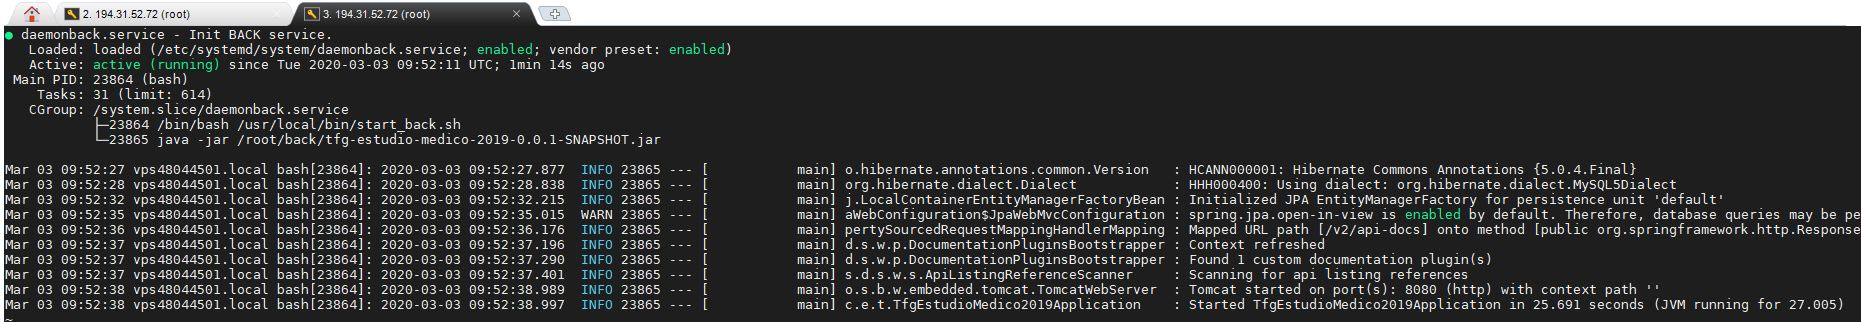
\includegraphics[width=1\textwidth]{images/serviciostart}
    \caption{Estado servicio}
    \end{figure}
    
    
    


    
    \section{Base de Datos}
    Para desplegar la base de datos en la web, se utilizó un servicio que ofrece Hostinger para desplegar bases de datos MySQL. 
    \newline 
    A través de PhpMyAdmin y con la opción de generar la base de datos automáticamente al ejecutar un proyecto Java Spring con JPA, se generó la siguiente base de datos:
    
     \begin{figure}[h]
    \centering
     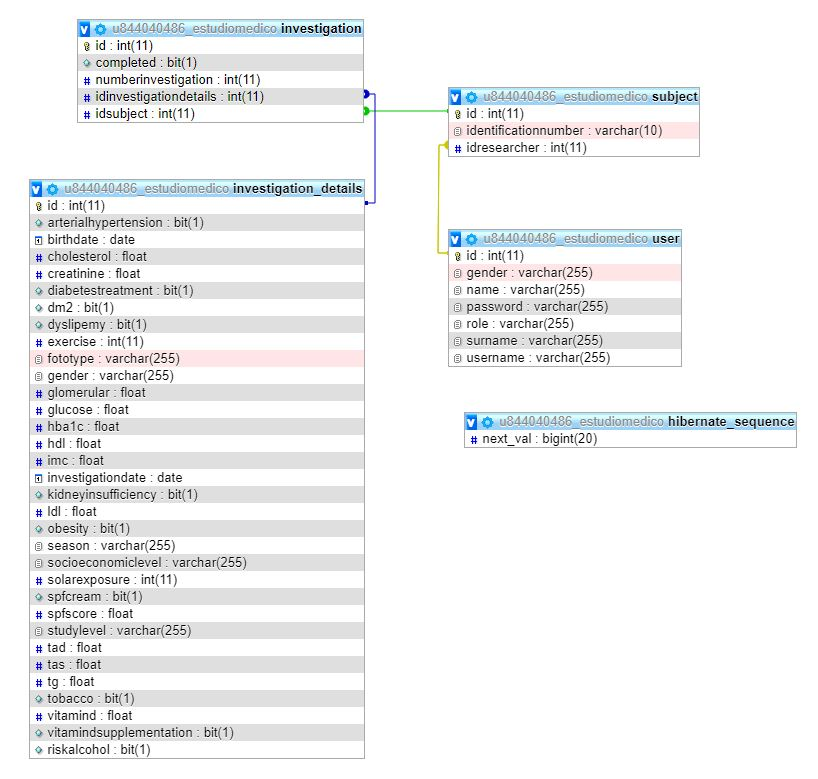
\includegraphics[width=1\textwidth]{images/modelodatos}
    \caption{Modelo de datos generado en PhpMyAdmin}
    \end{figure}
    
    

    \chapter{Resultados}
    \section{Simulación de resultados}
    \subsection{Suposiciones}
    \subsection{Modelos}
    \section{Resultados preliminares}
    \section{Resultados postprocesados}
    \subsection{Valores atípicos}
    \subsection{Correlaciones}
    
    

    \bibliographystyle{unsrt}
    \bibliography{references}
    
\end{document}